\input{E:/Blaok/Works/LaTeX/MATLAB.tex}

\begin{document}
\title{连连看大作业}
\author{池雨泽}
\maketitle
\section{制作自己的连连看}
\subsection{}
\noindent\ding{125}{\CJKfamily{kai} 在MATLAB环境下,设置当前路径为linkgame,运行linkgame(打开linkgame.fig 或右键linkgame.p点“运行”),熟悉游戏。(上述程序己经过MATLAB2010b以上版本的测试。)
}\ding{126}
\par 可以正常游戏。

\subsection{}
\noindent\ding{125}{\CJKfamily{kai}注意linkgame目录下有个detect.p,它的功能是检测块是否可以消除。 现在请你把它移动到其他文 件夹或删掉! 然后把linkgame\\reference 目录下的detect.m复制到linkgame目录下。 detect.m文件中 是detect函数,函数以图像块的索引矩阵与要判断的两个块的下标为输入,如果两个块能消掉则 输出1,否则输出0。 请根据文件中的注释提示,实现判断块是否可以消除的功能。 写完后再次运 行linkgame,检验游戏是否仍然可以正确运行,当你的程序的判断结果有误时,在游戏界面右下角 会有提示。(注意:当detect.p 文件存在时,detect.m 文件将不会被执行,所以测试时一定要移 走detect.p文件。)}\ding{126}
\par 这部分比较简单,只要按照提示实现功能即可。具体地,首先判断两个块儿是否一致,这是我开始时忽略的一点。若两块一致,则按拐弯次数不同分别判断。其中,直线相连由于被调用次数较多,我放在了单独的函数当中。一次拐弯相连是以交叉点为媒介,分别判断是否直接相连。两次拐弯需要包括在界外的情况,简单起见我直接扩展了游戏区域,然后扫描所有水平线和竖直线,以两个交叉点为媒介判断是否相连。一旦判断相连,立即返回true。否则,默认返回false。
\subsection{}
\noindent\ding{125}{\CJKfamily{kai}你一定发现了“外挂”模式,是不是很有趣?逐一自动消除所有的块的功能是由link 目录的omg.p实 现的。 现在请你把它也删掉! 然后把link\\reference目录下的omg.m复制到link目录下。 omg.m文件的 注释中对输入输出变量做了详细说明,请以这个文件为基础,实现逐一自动消除所有块的功能。(同 上题要移走omg.p文件。)写完后再次运行linkgame,检验自动模式是否正确。(在自动点击过程中可 接F12终止。)}\ding{126}
\par 这部分算法我有许多思路。比如,可以遍历每个方块,每次再遍历寻找可能的消除。假设判定两个方块这样复杂度将为块数的立方,太高。也可以从某个位置开始启发式查找,比如从边缘开始寻找可消除的方块对,然后在附近移动画线不断消除,这种方法实现比较复杂,但可能是最块的方法。我使用的方法是模拟人类解连连看,先选中某种图形,找出该图形的所有位置,查看两两之间能否消除,消除以后重新选择图形,循环往复。这种方法实际浪费了大量循环,但实现较为方便。像人类一样,选择的图形是随机的。

\section{攻克别人的连连看}
\subsection{}
\noindent\ding{125}{\CJKfamily{kai}在MATLAB环境下,将路径设置到process文件夹下。对游戏区域的屏幕截图(灰度图像) graygroundtruth进行分割,提取出所有图像分块。  在一个figure中用subplot方式按照原始顺序绘出所 有图像分块。}\ding{126}
\par \begin{center}
\includegraphics[width=\textwidth]{A4_2_1.eps}\end{center}

\subsection{}
\noindent\ding{125}{\CJKfamily{kai}对摄像头采集的图像(灰度图像)graycapture,参考第1题要求进行处理。讨论:和干净图像相比,被噪声污染的图像给分块带来了什么样的困难?
}\ding{126}
\par \begin{center}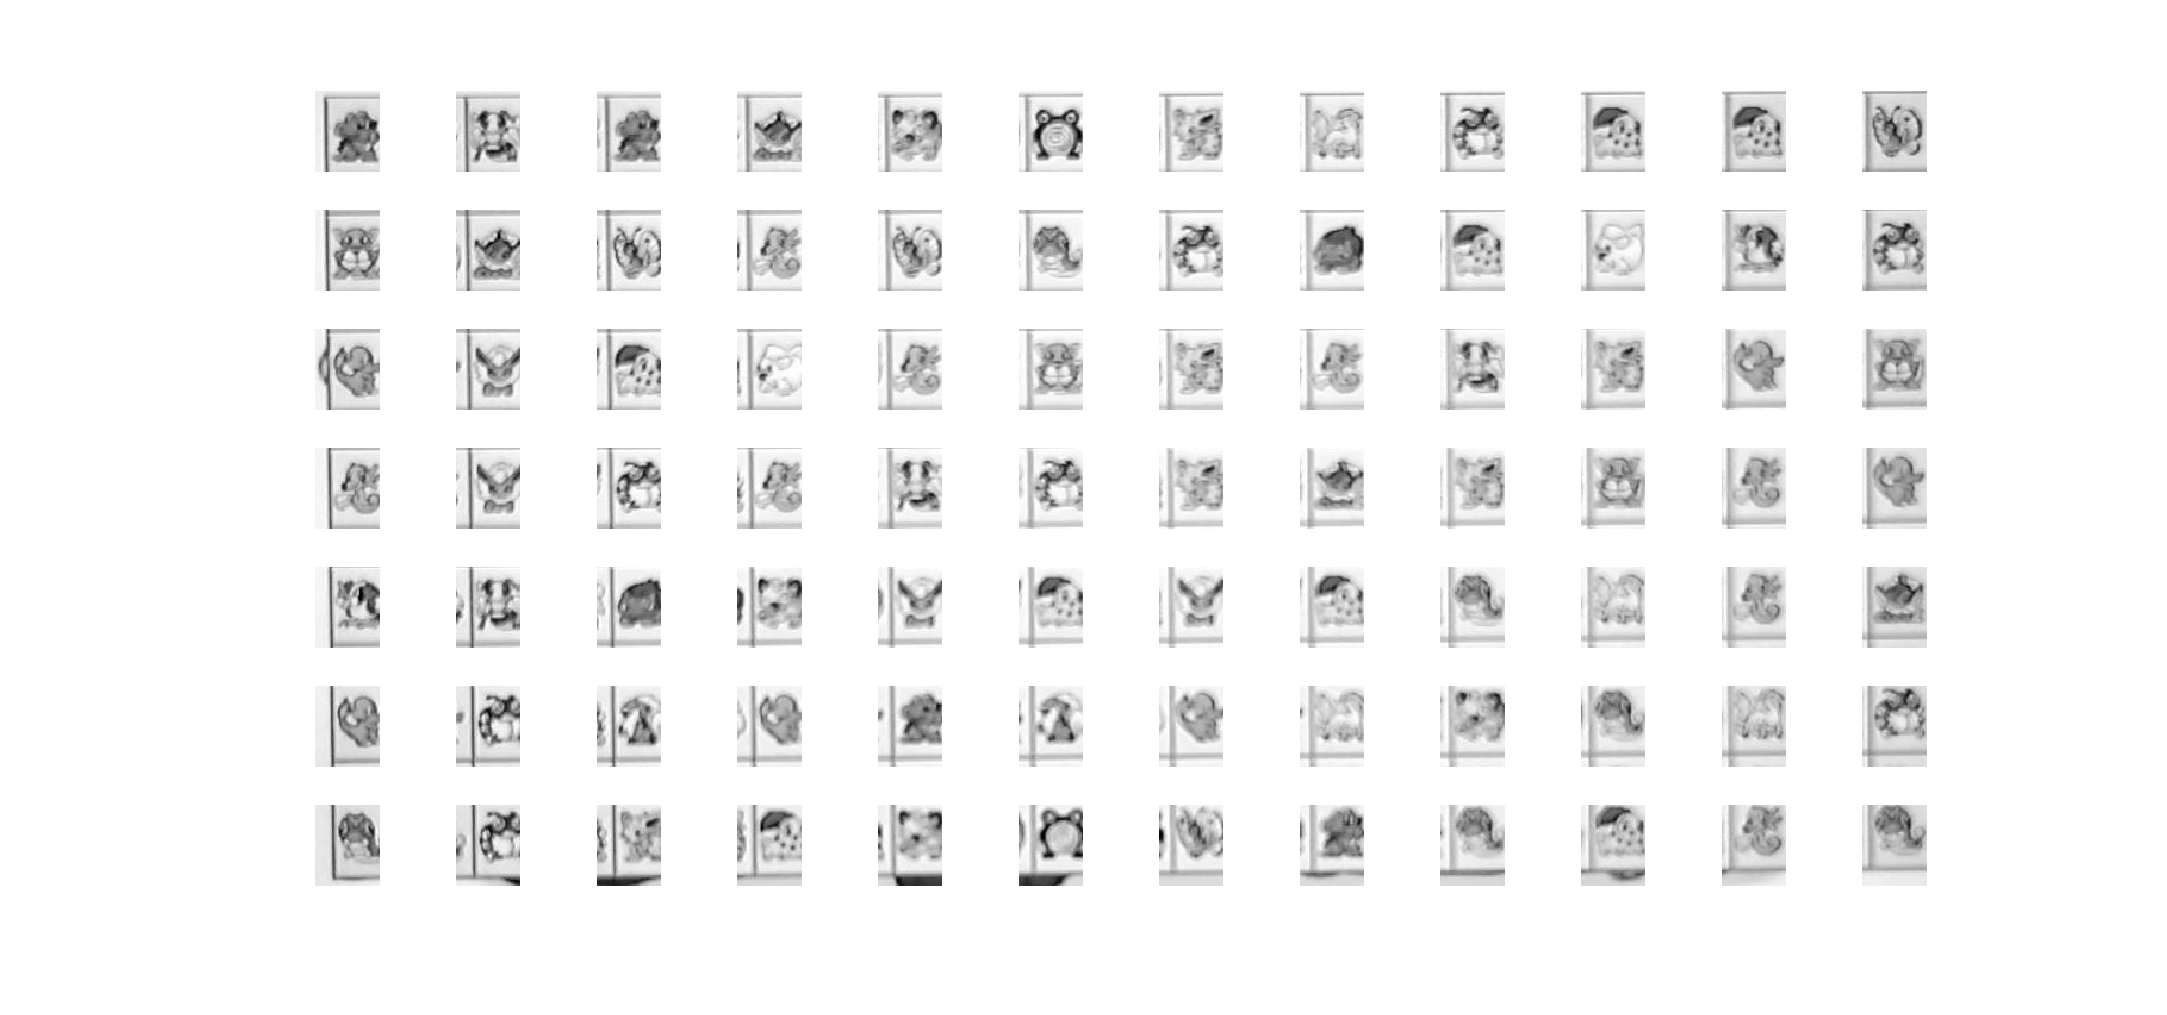
\includegraphics[width=\textwidth]{A4_2_2.eps}\end{center} 有噪声的图像周期性仍较好,但由于图像方向可能并不竖直,会造成无法合理分割图像,每一块儿都不可避免地包括其他部分。

\subsection{}
\noindent\ding{125}{\CJKfamily{kai}在第2题基础上,计算所有图像分块的两两相似性,选出最相似的十对图像块。 在一个figure中绘出, 并显示其相似性度量值。(建议先利用graygroundtruth测试代码的正确性,然后再用graycapture完成本题。)}\ding{126}
\par 这一部分耗时最久。一开始,我采用了直接两两做卷积的方法,使用的是内置的conv2函数,其性能比较好。但是,其结果并不好,经过思考,有几点原因:第一,卷积操作会反转图像,因此卷积结果并不能反映二者相关性。经过Google的搜索,我找到了xcorr2函数,计算的是二维的相关,解决了该问题;第二,卷积操作会在边缘引入奇怪的边缘效应,如果两个图像大小相同,因其求和范围不同,卷积结果必然中间大四周小,两两卷积并没有意义。在搜集资料和思考的过程中,我参考了Google得到的有关图像截取的资料,将相关运算作用在大小不同的两个图像上,即将每个块分别与全图做卷积,改进很明显;第三,卷积操作没有归一化,图像的绝对大小影响卷积结果。最终,我使用了normxcorr2函数来直接得到归一化以后的结果。
\par 此外,关于程序的性能,目前的性能对于graycapture在我的笔记本电脑上运行大概需要十几秒,其中绝大部分是花在了计算相关系数上面。在编写和调试的过程中我曾尝试自己写计算相关性的代码,但由于性能严重不如内置函数,很快我不得不放弃。因为一步连连看需要几分钟甚至半小时,实在太不符合我们的预期了。
\par 最终运行得到的结果如下
\par \begin{center}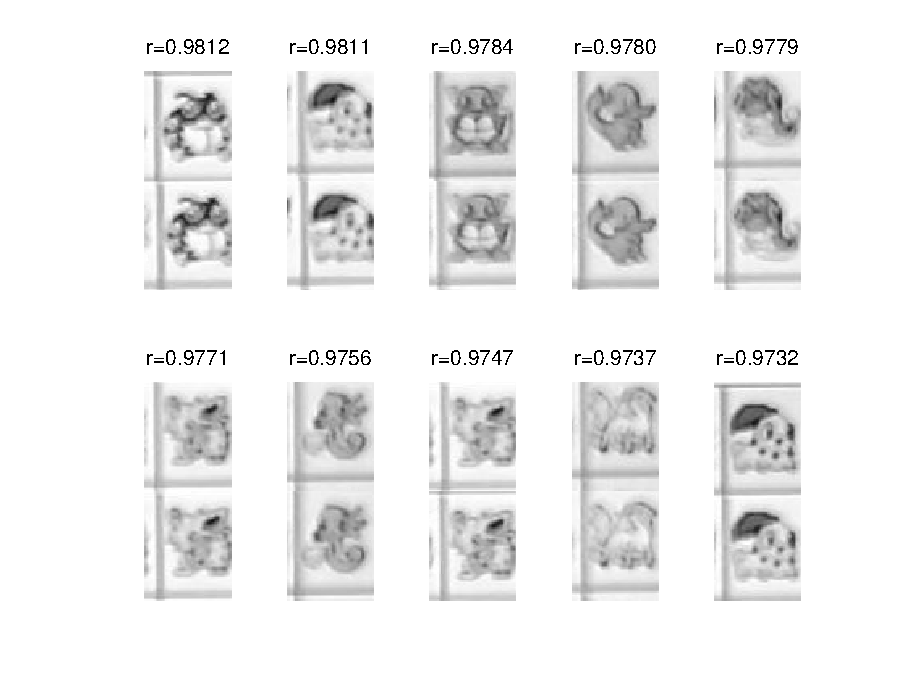
\includegraphics[width=\textwidth]{A4_2_3.eps}\end{center}

\subsection{}
\noindent\ding{125}{\CJKfamily{kai}在第3题基础上,找出相似度最大却不是同一种精灵的十对图像块。 在一个figure中绘出,并显示其相
似性度量值。  讨论:这个结果和你的主观感受一致吗?}\ding{126}
\par 结果如下
\par \begin{center}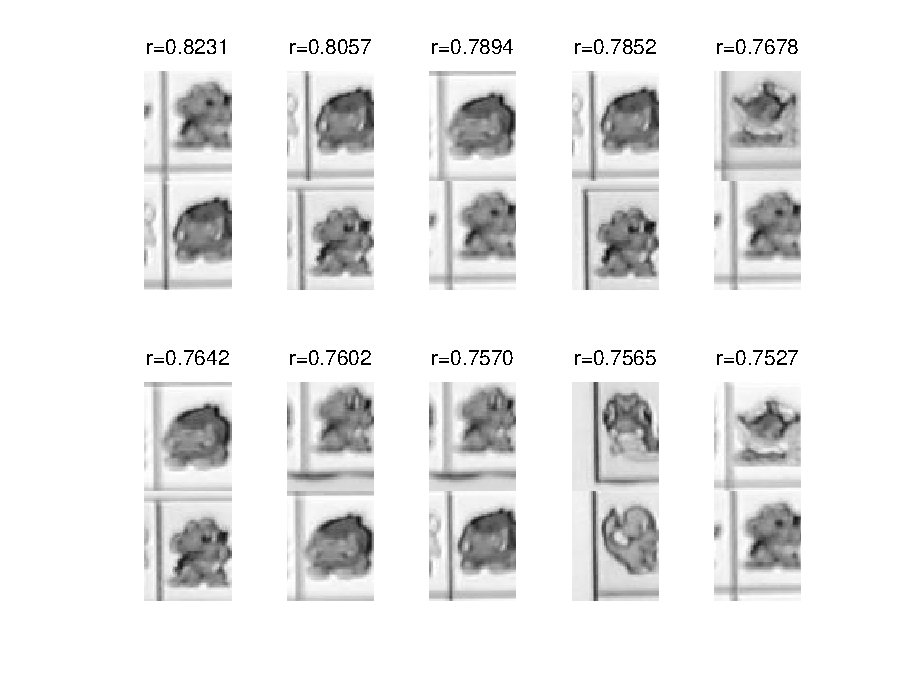
\includegraphics[width=\textwidth]{A4_2_4.eps}\end{center}
\par 与机器的比较稍有不同,人类可以轻易辨认出这十对图像并不是同一种小精灵。但仔细观察,他们两两之间的确存在相当大的相似性,特别是整体的灰度上非常相似。注意到计算得到的相关系数很低,这也说明机器也是在非常不想像的图像中选出了共同之处最多的十对,从这个意义上讲,这个结果是符合主观感受的。

\subsection{}
\noindent\ding{125}{\CJKfamily{kai}在第3题基础上,将游戏区域映射为索引值的数组,并列出索引值和图像分块的对照关系表。讨论:你可以将全部图像分块正确映射到其索引值吗?哪些分块无法正确映射?为什么?}\ding{126}
\par 可以全部正确映射,如下。
\par \begin{center}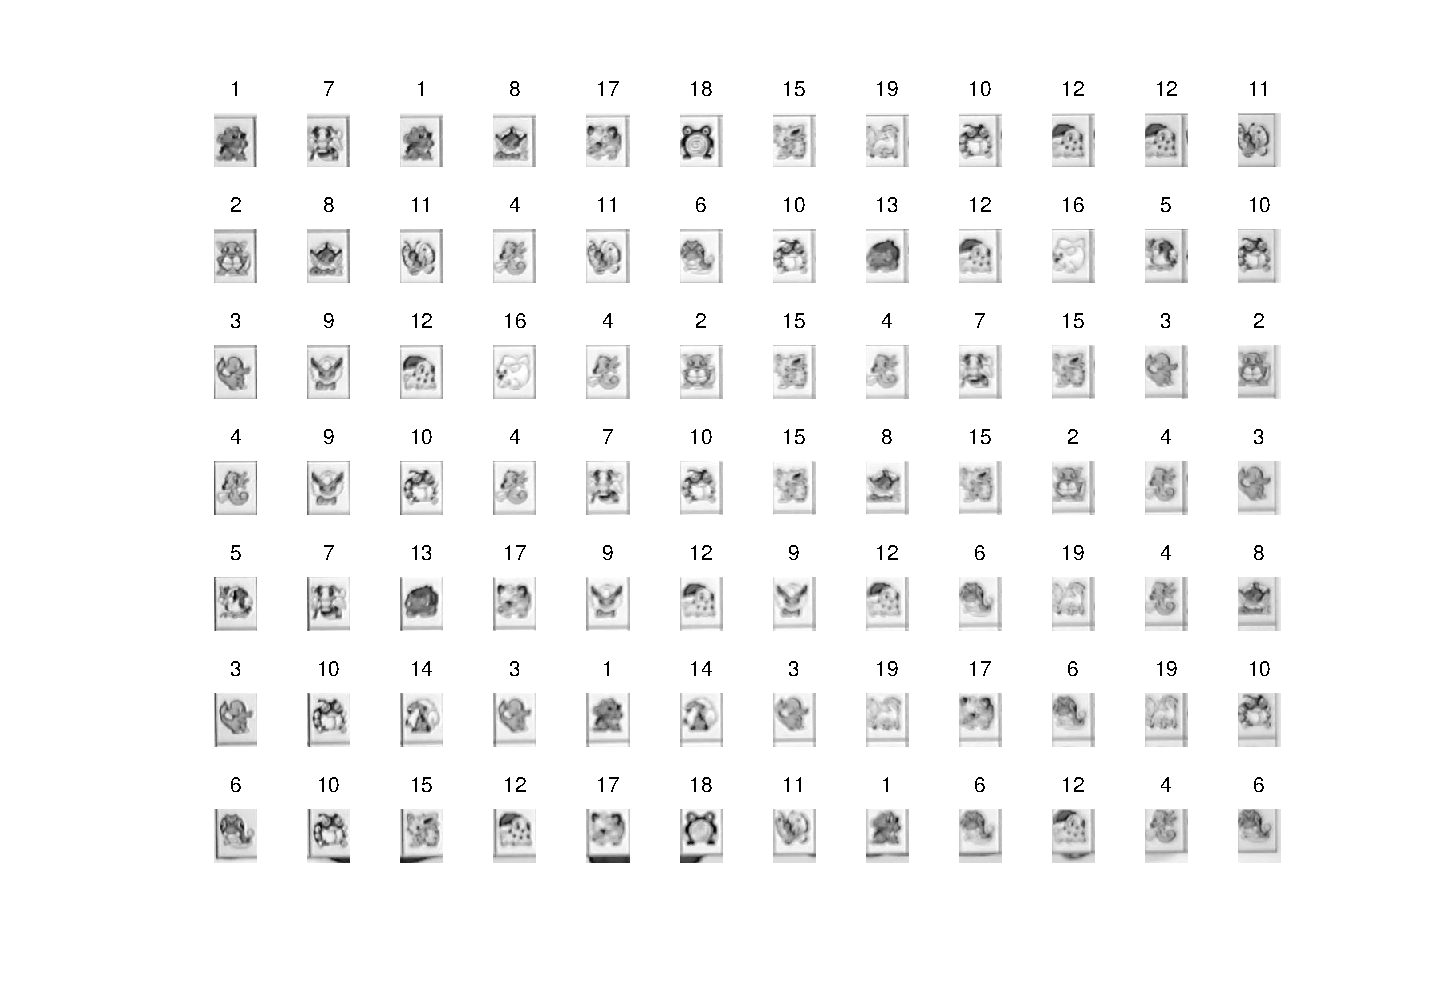
\includegraphics[width=\textwidth]{A4_2_5.eps}\end{center}



\subsection{}
\noindent\ding{125}{\CJKfamily{kai}在上述工作基础上,设计实现一个模拟的自动连连看。对摄像头采集的图像(灰度图像)graycapture进行分块并找出最相似的一对可消除分块后,将这图片上两个块的位置设为黑色或其他特定颜色(即模拟消除操作),并将图片展示在figure上。 然后继续找出下一对可消除的分块并模拟消除,直至消除所有的分块或找不到可消除的分块对。设计一种方法验证并展示上述工作的正确性。}\ding{126}
\par 我验证的方法是运行程序然后盯着屏幕看消除是否正确……结果非常理想,可以正确消除。过程我录制为视频A4\_2\_6.mp4。

\subsection{}
\noindent\ding{125}{\CJKfamily{kai}(选做)对摄像头采集的彩色图像colorcapture,重做第2至6题。 注意不能简单将彩色图变换为灰度图 后直接处理。 你的方法如何利用颜色信息?利用颜色信息是否可大幅提高正确率?(提示:1、图像处理大作业里讲过的彩色直方图;2、对X-Y-RGB三维张量做匹配滤波。)}\ding{126}
\par 结果如下(第六小问结果录制为视频A4\_2\_7.mp4):
\par \begin{center}\includegraphics[width=\textwidth]{A4_2_7_2.eps}\end{center}
\par \begin{center}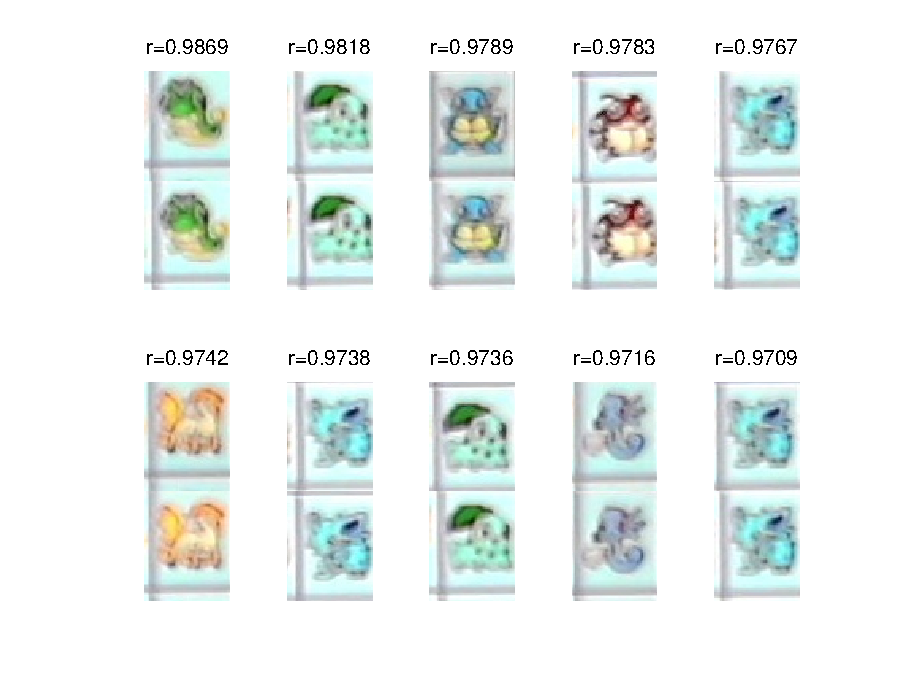
\includegraphics[width=\textwidth]{A4_2_7_3.eps}\end{center}
\par \begin{center}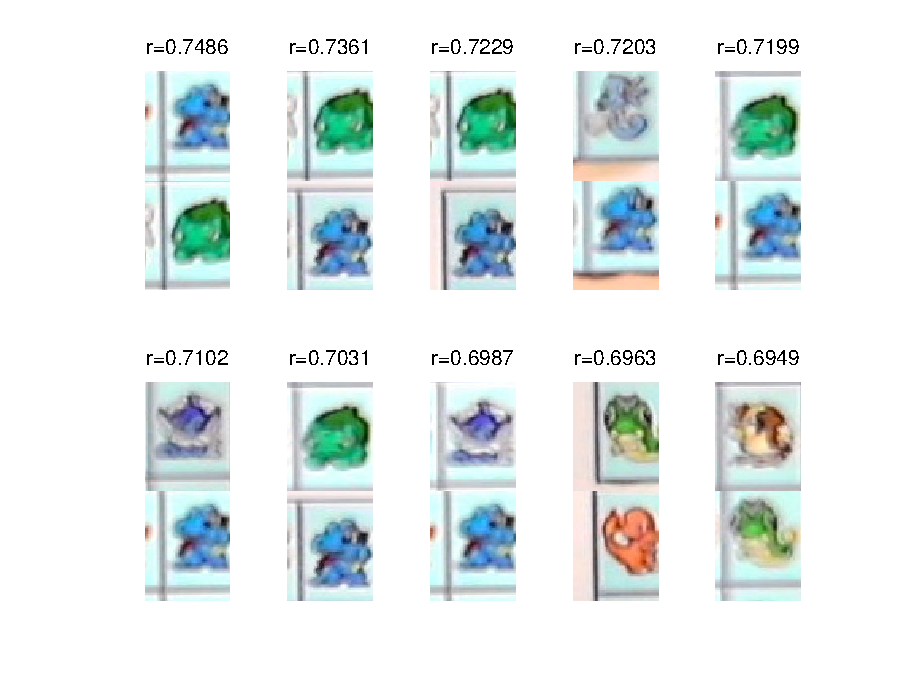
\includegraphics[width=\textwidth]{A4_2_7_4.eps}\end{center}
\par \begin{center}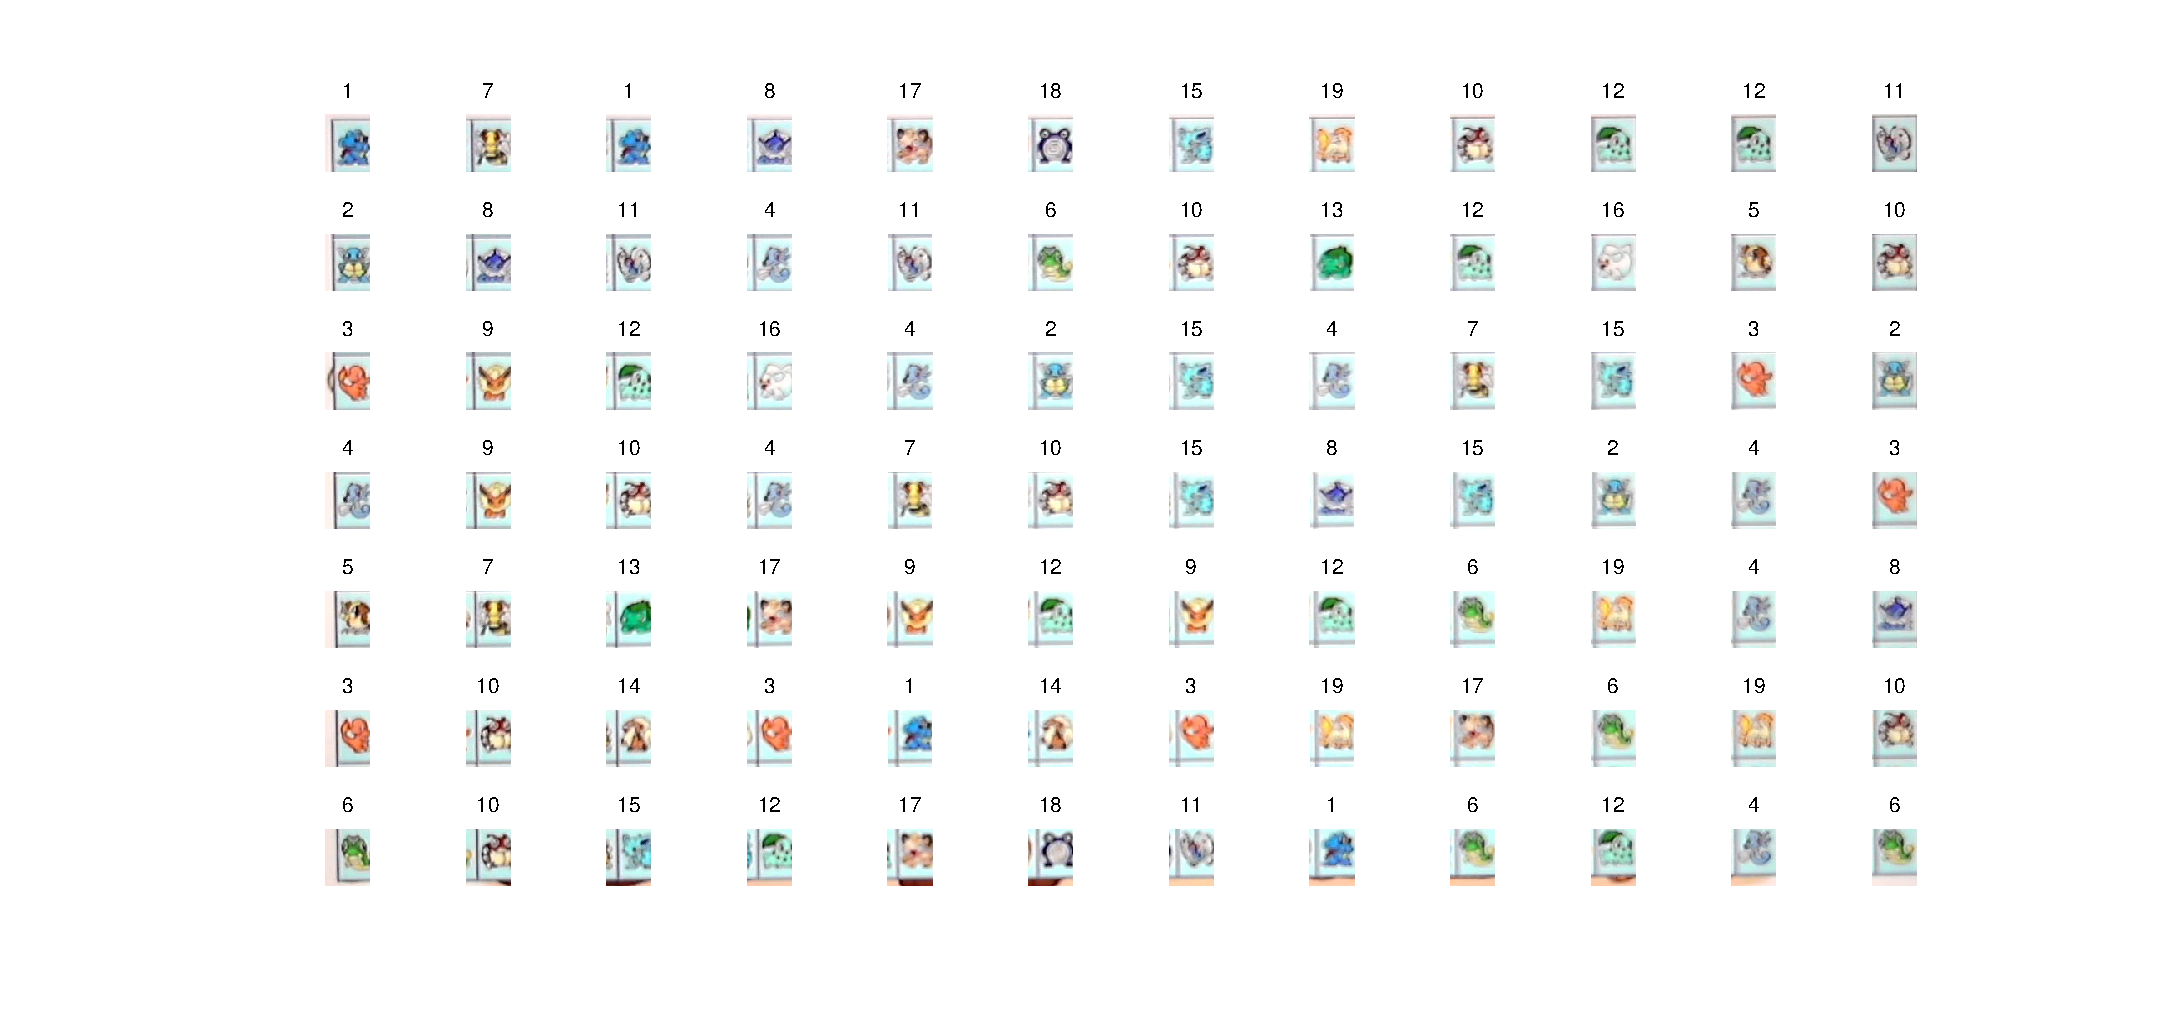
\includegraphics[width=\textwidth]{A4_2_7_5.eps}\end{center}
\par 我采用的技术主要是分层处理各个色彩分量。在分块时,对三个颜色分量分别处理,得到的参数做平均作为结果。在匹配时,以三个颜色分量相关系数的方均根归一化作为相关系数。结果方面,使用与此前略微不同的阈值,可以得到完全正确合理的结果。由于原来的结果已经完全正确,无法讨论颜色是否提高了正确率,但从信息量的角度,颜色无疑会增加判断的准确率。

\subsection{}
\noindent\ding{125}{\CJKfamily{kai}(选做)在上述工作基础上,设计实现一个真实的自动连连看。 主程序process/linkgame.p己经完成, 它首先采集摄像头的图像并保存为realcapture.jpg,然后调用ai.m,根据ai.m的输出参数step中指定的位置,利用按键精灵进行鼠标点击,完成一次操作。其中ai.m是需要你补全的文件。ai.m用来实现处理 图像realcapture.jpg,找出一对可消除分块,并把要消除的块的下标保存到step中输出(没有可消除的块则step = 1),输入输出格式在文件注释中有详细解释。 你可以使用process/reference/camera.m中 提供的代码调试摄像头位置。 完成后调用linkgame程序来测试。 完成本题需要使用一个分立的摄像头(并且要保证摄像头找到的绝大部分是游戏区域,否则你之前的程序可能无法处理),所以定为选做题。 但我非常希望同学们能够独立完成本题。完成后请录制一段自动游戏的视频,上传到学堂,让大家一 起分享你成功的喜悦!}\ding{126}
\par 这一部分调试整体上顺利,但过程中遇到不少坎坷。首先遇到的问题是摄像头。由于老师非常及时地公开了摄像头的代码,使我可以用IP摄像头获取图像并直接予以处理,这非常方便。其次是坐标的混乱。开始一段时间程序都可以输出坐标但按键精灵找不到正确的位置……经过反复检查发现坐标的横纵顺序是颠倒的。还有一个问题是采光,晚上调试的正确率非常不靠谱,导致不得不等等早上录制。
\par 算法方面,由于我匹配所需的时间较长,因此我采用的策略是首次将全部步骤计算出来,以后每次使用已经计算好的结果。录制方面,我直接以手机作为IP摄像头录制,录制现场的截图如下。录制结果保存为A4\_2\_8.mp4。
\par \begin{center}\includegraphics[width=\textwidth]{A4_2_8.eps}\end{center}
\par 条件比较艰苦,视频效果不是很好,请见谅。





\XeTeXdefaultencoding GBK
\lstinputlisting{linkgame/detect.m}
\lstinputlisting{linkgame/omg.m}
\lstinputlisting{A4_2_1.m}
\lstinputlisting{A4_2_2.m}
\lstinputlisting{A4_2_3.m}
\lstinputlisting{A4_2_4.m}
\lstinputlisting{A4_2_5.m}
\lstinputlisting{A4_2_6.m}
\lstinputlisting{A4_2_7.m}
\lstinputlisting{process/ai.m}
\lstinputlisting{process/detect.m}
\lstinputlisting{process/user_camera.m}
\lstinputlisting{process/prefourier.m}
\lstinputlisting{process/cal.m}
\XeTeXdefaultencoding auto
\end{document}
